%!TEX root=../bulletin.tex
%\section{Instant Insights from Raw Data}
\section{Introduction}
\label{sec:intro}

% the problem at large
Driven by the promise of big data analytics, enterprises gather data 
at an unprecedented rate that challenge state-of-the art analytics 
algorithms~\cite{data_growth}.
%
Decision support systems used in industry, and modern-day analytics 
involve interactive data exploration, visual analytics, 
aggregate dashboards, and iterative machine learning workloads. Such applications, 
rely heavily on efficient data access, and require 
real-time response times irrespective of the data size. 
%
Besides the high volume of data, data analysis requires
combining information from multiple datasets of various data formats which are 
often inconsistent~\cite{data_quality,Karpathiotakis2016}.
Therefore, satisfying these requirements is a challenge
for existing database management systems.

% problem 1 (data preparation) introduction
To offer real-time support, database management systems require 
compute and data-intensive preprocessing operations which sanitize the 
data through data loading and cleaning, and enable efficient data 
access through tuning. 
% problem 2 (static decisions) introduction
These data preparation tasks rely heavily on assumptions over 
data distribution and future workload. 
However, real-time analytics applications access data instantly after 
its generation and often workloads are constantly shifting based on 
the query results~\cite{Chen2012a}. Thereby, making a priori 
static assumptions about data or queries may harm query 
performance~\cite{Agrawal2004,Chaudhuri1997}.

% What is data preparation?
% Loading
Data preparation involves several steps of processing until raw data
is transformed
into a form that fits data analysis.
To enable queries that combine a variety of data formats, such as
relational, or semi-structured hierarchical formats which have become 
the state-of-the-art for data exchange, data scientists rely on 
database management engines which offer a broad-range of analysis 
operations.  
% Loading
To overcome this heterogeneity of data formats, database management 
systems perform \textit{data loading} which transforms raw data into 
a single relational data format to allow for more flexibility in
the operations that users can execute.
%which reduces data access cost.
% Cleaning
As the data collected by the application is often a result of 
combining multiple, potentially erroneous sources, it 
contains inconsistencies and duplicates. To return correct 
results, database management systems 
must recognize such irregularities and remove them through 
\textit{data cleaning} before analyzing the data.
% Tuning
Finally, to improve query performance and enable near real-time query 
responses, database management systems avoid or reduce unnecessary 
data access by \textit{tuning access paths} (e.g., indexes) over the 
dataset.
\begin{figure*}[t]
	\begin{center}
		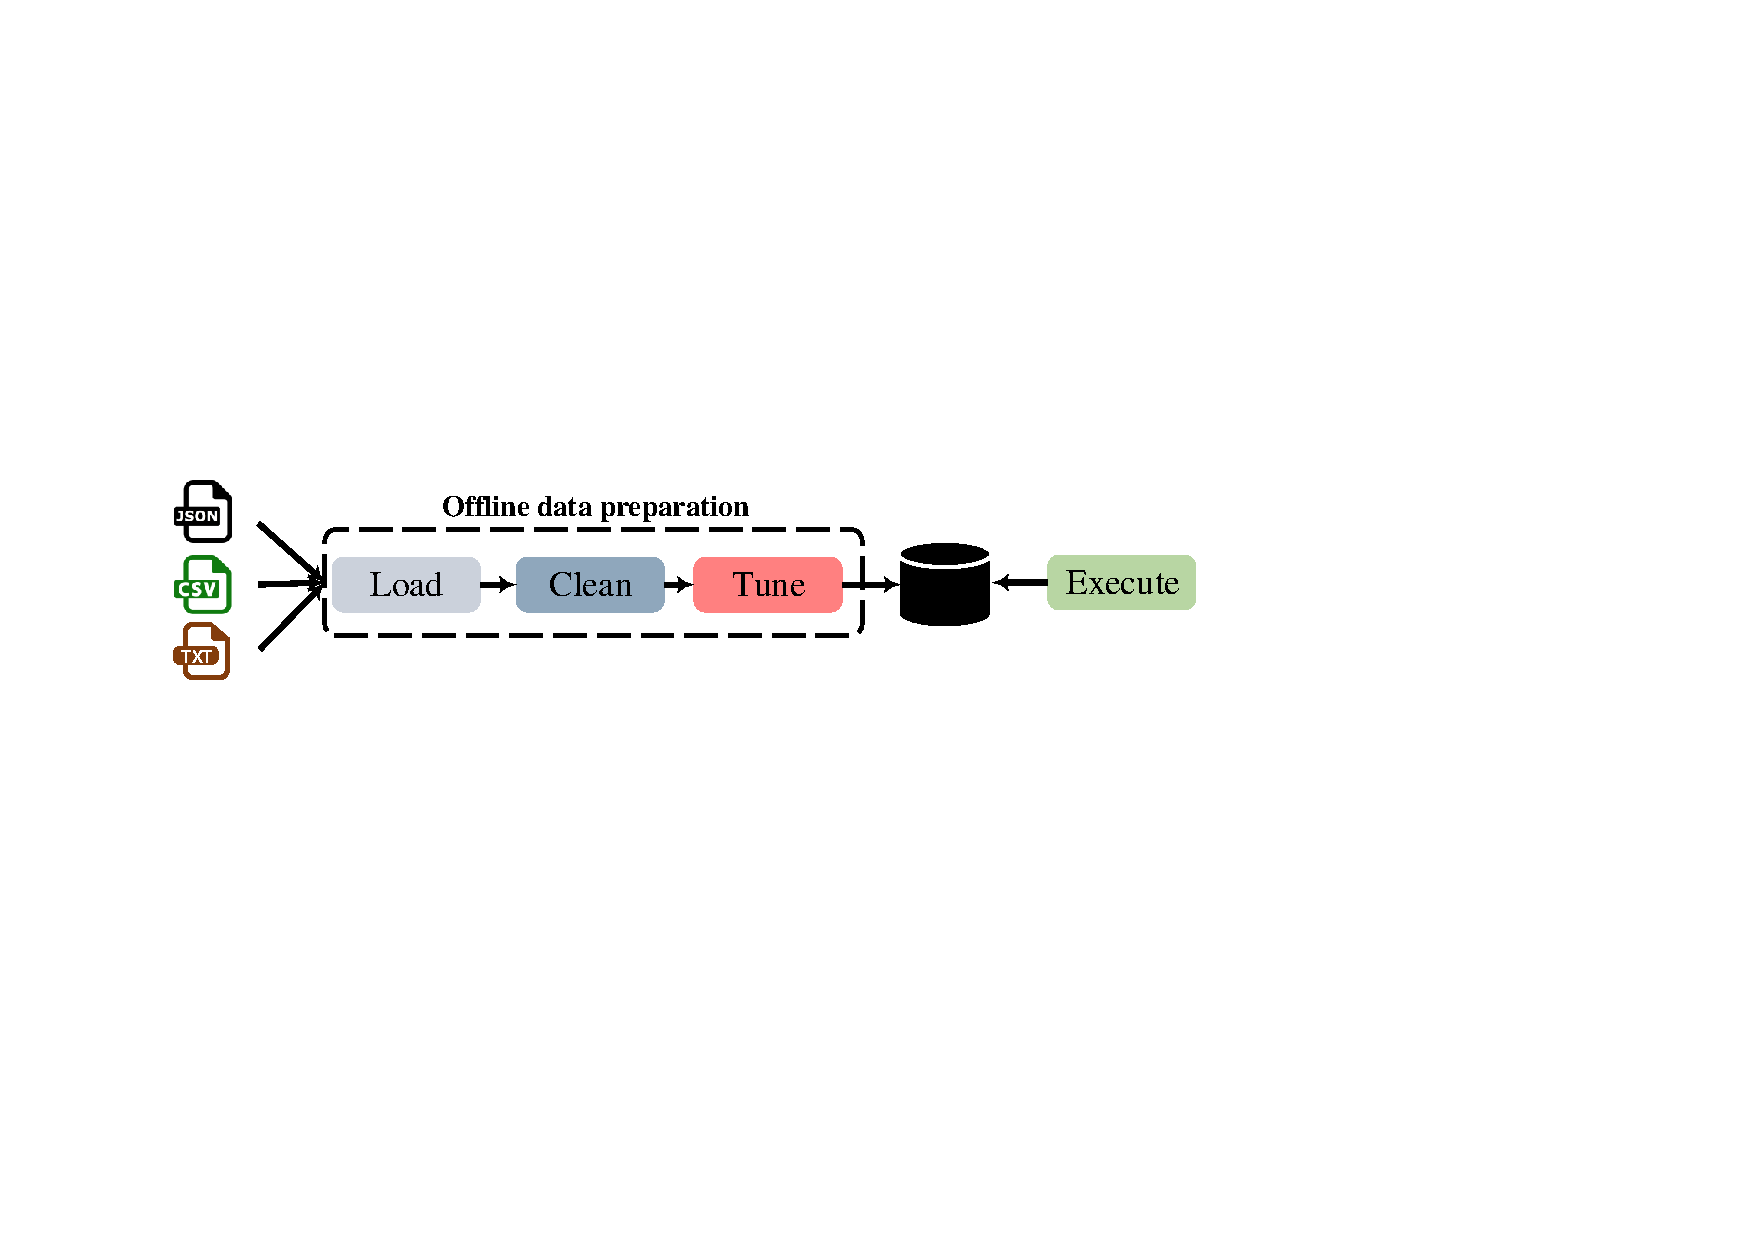
\includegraphics[page=1,width=0.7\columnwidth]{figs/data-preparation-offline}
%		\caption{Data Processing alternatives.}
		\caption{Data Processing pipeline.}
		\label{fig:alternatives}
	\end{center}
	\vspace{-2em}
\end{figure*}
%
\fref{fig:alternatives} presents the data pipeline of a 
state-of-the-art data analytics framework. The data to be analyzed is collected 
from a variety of sources, and might appear in various formats (e.g., XML, CSV, etc.). 
The multiple input formats are transformed into a single uniform format by loading
them into a DBMS. Then, to remove any inconsistencies cleaning operations are applied. Finally, 
a tuner builds access paths for 
efficient access. The final result is stored in a clean and tuned 
database, and is ready to receive query requests.

% re-cap and prepare for upcoming paragraphs
The preprocessing steps are exploratory and data-intensive, as they involve expensive operations, and highly depend on the data and the query workload. Data preparation tasks access the entire dataset multiple times: data loading results in copying and transforming the whole dataset into a common format. Cleaning tasks perform multiple passes over the data until they fix all the inconsistencies. Finally, to build indexes, an extra  traversal of the dataset is needed. Therefore, the increasing 
data volume limits the scalability of data preparation.
%
Furthermore,  the benefits of data preparation depend highly on the 
to-be executed workload. Data transformation and cleaning are only 
useful if the queries are data intensive and access the majority of 
data. Finally, tuning requires a priori knowledge of queries to decide 
upon the most efficient physical design.


\begin{wrapfigure}{L}{0.35\textwidth}
%		\centering
	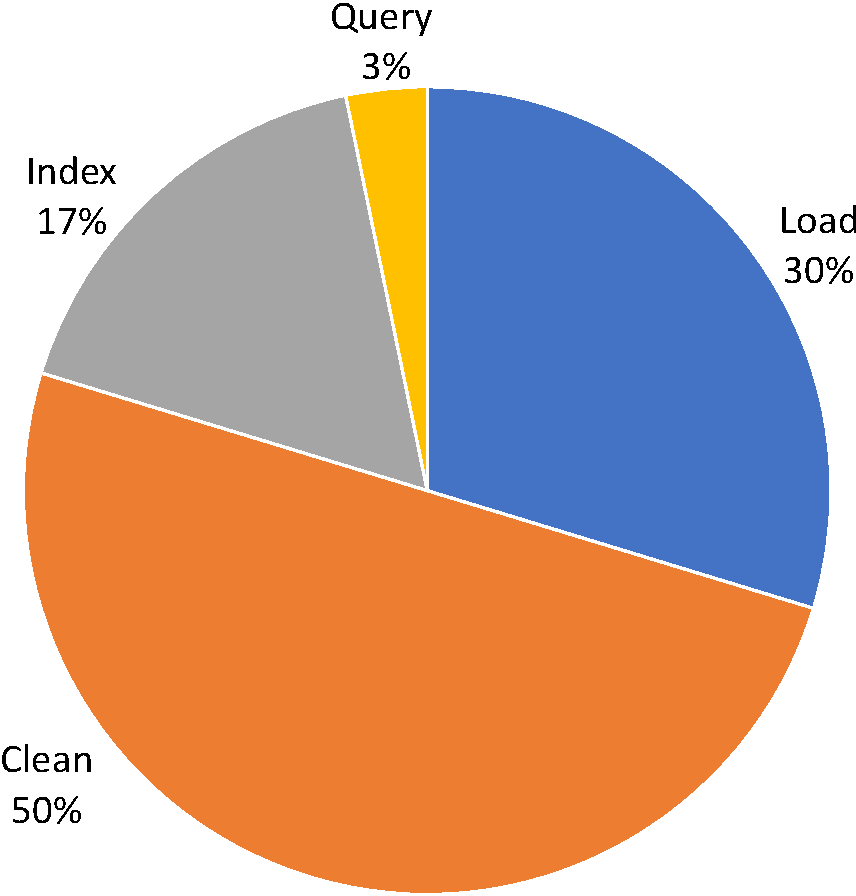
\includegraphics[width=0.34\columnwidth]{figs/breakdown_pie}	
	\caption{Cost of Data Preprocessing}
	\label{fig:preprocessing}
\end{wrapfigure}

% Tech problem 1: These are very expensive and take a very long time.
\Paragraph{Data preparation is time consuming} 
Due to the influx of data, data preparation becomes increasingly 
expensive. ~\fref{fig:preprocessing} demonstrates the breakdown of
the overall execution time of a typical data analysis scenario.
The breakdown corresponds to the time that a system requires to 
preprocess the data and execute a set of 10 queries. The execution 
time reported at 
each step is based on recent studies on loading, cleaning, and tuning 
\cite{buckley_new_2012,Olma2017a}.
Specifically, assuming an optimistic scenario in which data cleaning
corresponds to 50\% of the analysis time, then based on \cite{Olma2017a},
the rest 50\% 
is mostly spent on loading and tuning. The loading percentage may become even higher 
in the presence of non-relational data formats, such 
as XML, because a DBMS will have to flatten the dataset in order to 
load it. Query execution takes 3\% of the overall time. Therefore, 
data preparation incurs a significant overhead to data analysis.

% Insight 1: We don't need to do them on the whole data but only on 
%the parts that we care about.
Despite enterprises collecting and preparing 
increasingly larger amounts of data for analysis, often the effectively useful 
data is considerably smaller than the full 
dataset~\cite{scientific_data,Papadomanolakis2004}. 
The trend of exponential data growth due to intense data generation 
and data collection is expected to persist, however, recent studies 
of the data analysis workloads show that typically only a small 
subset of the data is relevant and ultimately used by analytical 
and/or exploratory workloads~\cite{Chen2012a}. 
Therefore, having to preprocess the whole dataset results in wasting
effort on data which are unnecessary for the actual analysis.
% Insight 2: Approximation
Furthermore, modern-day analytics, are increasingly tolerant to 
result imprecision. In many cases, precision to ``last decimal'' is 
redundant for a query answer. Quick approximation with some error 
guarantee is adequate to provide insights about the 
data~\cite{Cormode2012}.
Thus, using query approximation, one can execute analytical  queries  
over small samples of the dataset, and obtain approximate results 
within a few percents of the actual value \cite{Olma2019}.

\Paragraph{Ever Changing Workload}
Modern businesses and scientific applications require interactive 
data access, which is characterized by no or little a priori workload 
knowledge and constant workload shifting both in terms of projected 
attributes and selected ranges of the data.
% motivating example
For example, an electricity monitoring company continuously collects 
information about the current and aggregate energy consumption, and 
other sensor measurements such as temperature. To optimize 
consumption, the company performs predictive analytics over 
smart home datasets, looking for patterns that indicate energy 
request peaks and potential equipment downtime~\cite{IBM2012}. 
Analyses in this context start by identifying relevant 
measurements by using range queries and aggregations to identify 
areas of interests. The analysis focuses on specific data regions for 
a number of queries, but is likely to shift across the dataset to a 
different subset.
% we cannot predict what to prioritize and how to do this.
Due to the unpredictable nature of data analytics workloads, where 
queries may change depending on prior query results, applications
prepare all data for data access to avoid result inconsistencies. 
This preparation requires investment of time and resources into data 
that may be useless for the workload, thereby delaying data analysis.

\Paragraph{Adapt to Data and Workload}
% What do we propose as an approach: Adaptivity
To address the aforementioned shortcomings, we revisit the data processing
pipeline, and aim to streamline the process of extracting insights from data. 
We reduce 
the overall time of data analysis by introducing approaches which adapt
online to workload and dataset, which reduce the cost of each of the 
steps of data analysis from data collection to result.
Specifically, to reduce the cost of loading, we execute queries over 
raw data files \cite{Alagiannis2012a, 
Karpathiotakis2016,Karpathiotakis2015,Karpathiotakis2014}, to reduce 
the cost of data cleaning we piggy-back operations over query 
execution and we only sanitize data affected by the queries 
\cite{query_driven_cleaning}. Finally, to reduce the cost of tuning, 
we take advantage of data distribution as well as relaxed precision 
constraints of applications and adapt access paths online and as a
by-product of query execution to data and 
workload~\cite{Olma2017a,Olma2019}. 
\fref{fig:online-query-execution} demonstrates the revised data 
analysis process which weaves data preprocessing into query execution 
by adapting to the underlying data, as well as to the query workload.

% what is our design?
At the core of our approach lies \textit{in-situ} query processing, 
which allows the execution of declarative queries over external files 
without duplicating or ``locking'' data in a proprietary database 
format. 
% adapt to data formats
We extend \textit{in-situ} approaches 
\cite{Alagiannis2012a,Idreos2011} by treating any data format as a 
first-class citizen. To minimize query response times, we build a 
just-in-time query engine specialized for executing queries over 
multiple data formats. This approach removes the need for 
transforming and loading, while also offering low data access cost.
%
% adapt cleaning
To reduce the cost of data cleaning, we enhance query execution by 
injecting data cleaning operations inside the query plan. 
Specifically, we introduce a query answer relaxation technique which 
allows repairing erroneous tuples at query execution time. By 
relaxing the query answer, we ensure that the query returns all entities 
that may belong to the query result (e.g., no missing tuples).
%
% adapt access paths
Finally, similarly to data cleaning, building indexes over a 
dataset is becoming increasingly harder due to (i) shifting workloads 
and (ii) increasing data sizes which increase access path size as 
well.
The decision on what access paths to build depends on the expected 
workload, thus, traditional database systems assume knowledge of future 
queries. However, the shifting workload of modern data analytics can 
nullify investments towards indexing and other auxiliary data 
structures. Furthermore, access path size increases along with input 
data, thus, building precise access paths over the entire dataset 
limits the scalability of databases systems.
To address these issues, we adapt access paths to data 
distribution and precision requirements of the result. This enables 
building data structures specifically designed to take advantage of 
different data distributions and create data summaries requiring less 
storage space.

\begin{figure*}[t]
	\begin{center}
		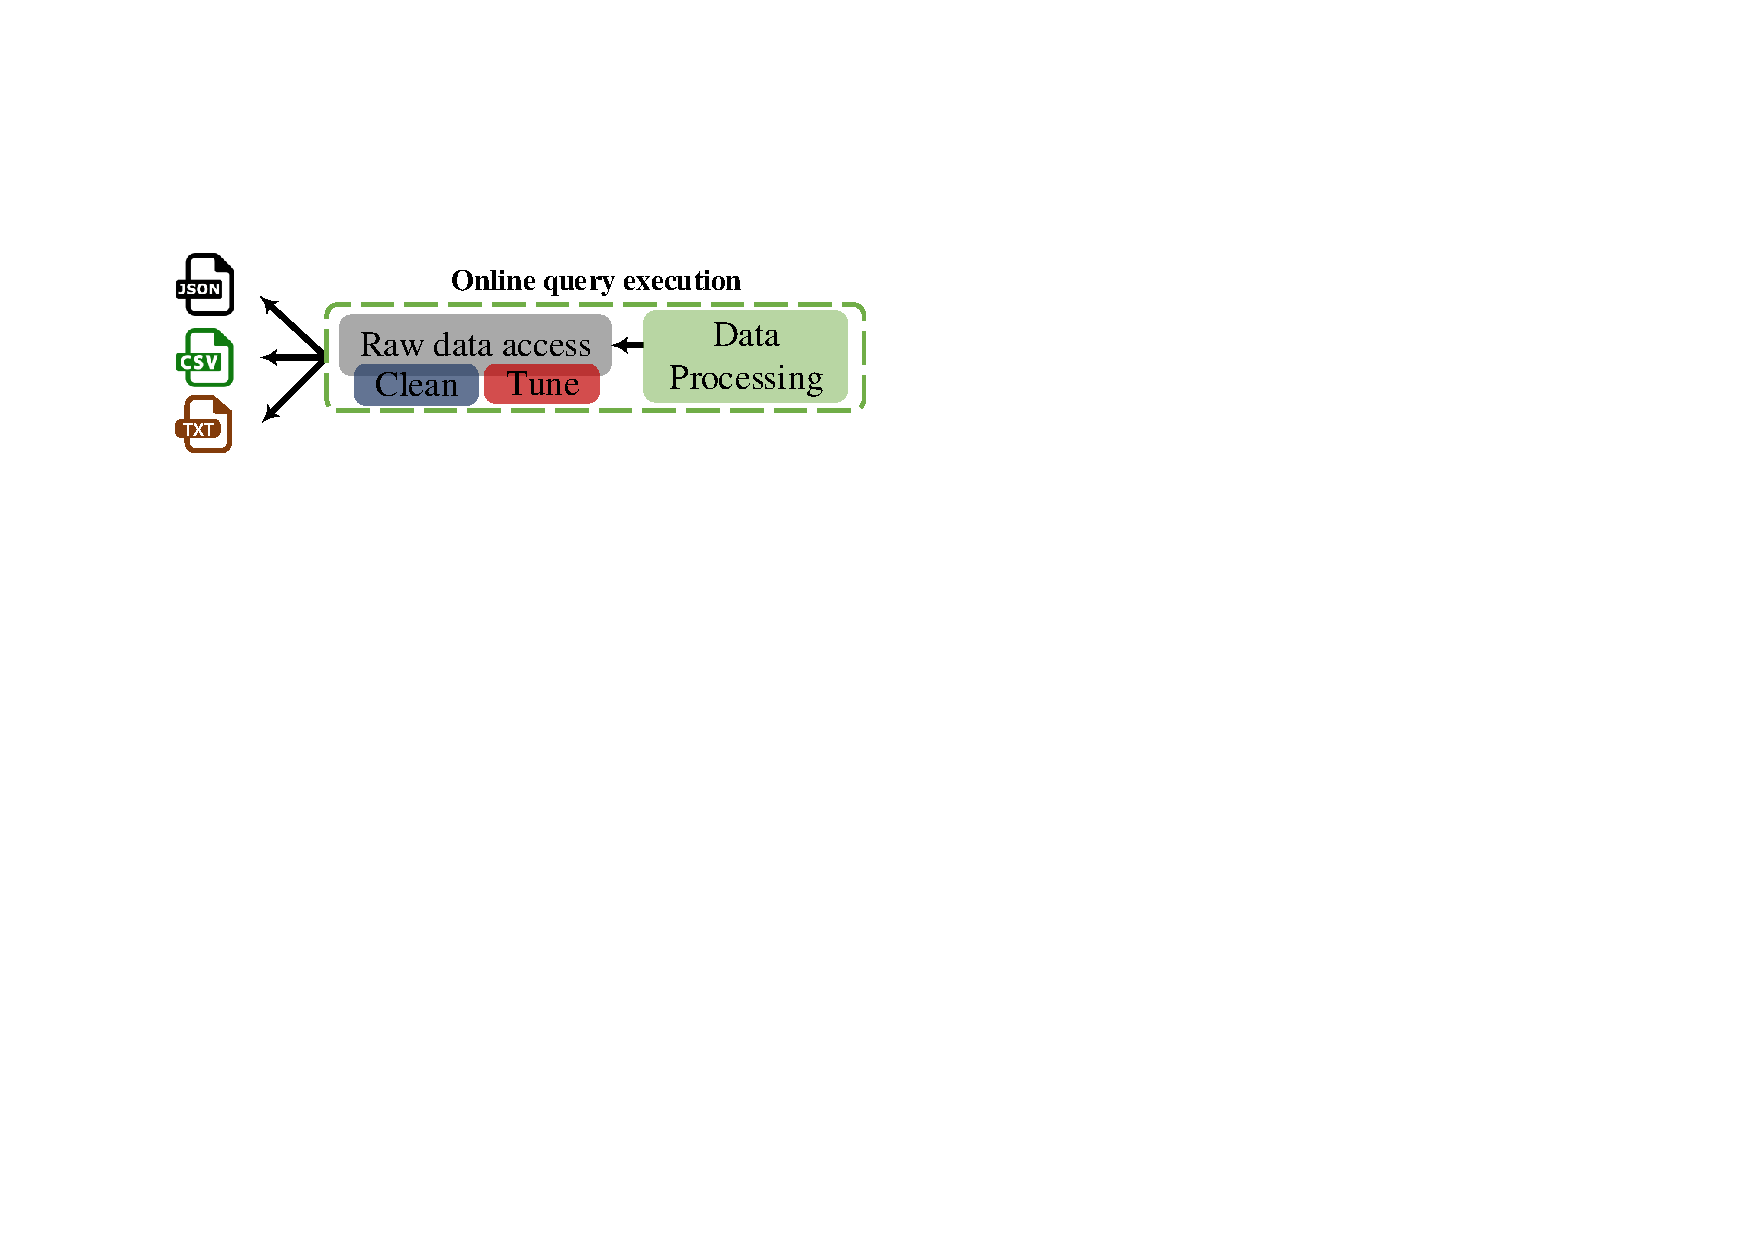
\includegraphics[page=1,width=0.5\columnwidth]{figs/query-execution-online}
		\caption{Integrating Cleaning and Tuning to Data Access.}
		\label{fig:online-query-execution}
	\end{center}
	\vspace{-2em}
\end{figure*}

In this paper we describe techniques that enable instant access to 
data irrespective of data format, and enable data cleaning and tuning 
without interrupting query execution. Each technique addresses a step 
in the preprocessing phase of data analysis, reducing the total 
data-to-insight time for users. Specifically, in~\sref{sec:proteus}, 
we describe the design behind our just-in-time query engine which 
enables efficient query execution despite data heterogeneity. 
In~\sref{sec:cleaning}, we demonstrate a novel approach to intertwine 
query execution with data cleaning through query answer relaxation. 
Our approach incrementally cleans only data that will be analyzed. 
In~\sref{sec:accesspaths}, we present our approach to adapt access 
paths online to data distribution and to precision requirements, as 
well as to available storage resources. Finally, 
in~\sref{sec:conclusion}, we conclude by highlighting techniques and 
related open problems for adaptive data management systems.